% Options for packages loaded elsewhere
\PassOptionsToPackage{unicode}{hyperref}
\PassOptionsToPackage{hyphens}{url}
%
\documentclass[
  10pt,
  letterpaper,
  DIV=11,
  numbers=noendperiod,
  twoside]{scrartcl}

\usepackage{amsmath,amssymb}
\usepackage{setspace}
\usepackage{iftex}
\ifPDFTeX
  \usepackage[T1]{fontenc}
  \usepackage[utf8]{inputenc}
  \usepackage{textcomp} % provide euro and other symbols
\else % if luatex or xetex
  \usepackage{unicode-math}
  \defaultfontfeatures{Scale=MatchLowercase}
  \defaultfontfeatures[\rmfamily]{Ligatures=TeX,Scale=1}
\fi
\usepackage{lmodern}
\ifPDFTeX\else  
    % xetex/luatex font selection
  \setmainfont[ItalicFont=EB Garamond Italic,BoldFont=EB Garamond
Bold]{EB Garamond Math}
  \setsansfont[]{Europa-Bold}
  \setmathfont[]{Garamond-Math}
\fi
% Use upquote if available, for straight quotes in verbatim environments
\IfFileExists{upquote.sty}{\usepackage{upquote}}{}
\IfFileExists{microtype.sty}{% use microtype if available
  \usepackage[]{microtype}
  \UseMicrotypeSet[protrusion]{basicmath} % disable protrusion for tt fonts
}{}
\usepackage{xcolor}
\usepackage[left=1in, right=1in, top=0.8in, bottom=0.8in,
paperheight=9.5in, paperwidth=6.5in, includemp=TRUE, marginparwidth=0in,
marginparsep=0in]{geometry}
\setlength{\emergencystretch}{3em} % prevent overfull lines
\setcounter{secnumdepth}{3}
% Make \paragraph and \subparagraph free-standing
\ifx\paragraph\undefined\else
  \let\oldparagraph\paragraph
  \renewcommand{\paragraph}[1]{\oldparagraph{#1}\mbox{}}
\fi
\ifx\subparagraph\undefined\else
  \let\oldsubparagraph\subparagraph
  \renewcommand{\subparagraph}[1]{\oldsubparagraph{#1}\mbox{}}
\fi


\providecommand{\tightlist}{%
  \setlength{\itemsep}{0pt}\setlength{\parskip}{0pt}}\usepackage{longtable,booktabs,array}
\usepackage{calc} % for calculating minipage widths
% Correct order of tables after \paragraph or \subparagraph
\usepackage{etoolbox}
\makeatletter
\patchcmd\longtable{\par}{\if@noskipsec\mbox{}\fi\par}{}{}
\makeatother
% Allow footnotes in longtable head/foot
\IfFileExists{footnotehyper.sty}{\usepackage{footnotehyper}}{\usepackage{footnote}}
\makesavenoteenv{longtable}
\usepackage{graphicx}
\makeatletter
\def\maxwidth{\ifdim\Gin@nat@width>\linewidth\linewidth\else\Gin@nat@width\fi}
\def\maxheight{\ifdim\Gin@nat@height>\textheight\textheight\else\Gin@nat@height\fi}
\makeatother
% Scale images if necessary, so that they will not overflow the page
% margins by default, and it is still possible to overwrite the defaults
% using explicit options in \includegraphics[width, height, ...]{}
\setkeys{Gin}{width=\maxwidth,height=\maxheight,keepaspectratio}
% Set default figure placement to htbp
\makeatletter
\def\fps@figure{htbp}
\makeatother
% definitions for citeproc citations
\NewDocumentCommand\citeproctext{}{}
\NewDocumentCommand\citeproc{mm}{%
  \begingroup\def\citeproctext{#2}\cite{#1}\endgroup}
\makeatletter
 % allow citations to break across lines
 \let\@cite@ofmt\@firstofone
 % avoid brackets around text for \cite:
 \def\@biblabel#1{}
 \def\@cite#1#2{{#1\if@tempswa , #2\fi}}
\makeatother
\newlength{\cslhangindent}
\setlength{\cslhangindent}{1.5em}
\newlength{\csllabelwidth}
\setlength{\csllabelwidth}{3em}
\newenvironment{CSLReferences}[2] % #1 hanging-indent, #2 entry-spacing
 {\begin{list}{}{%
  \setlength{\itemindent}{0pt}
  \setlength{\leftmargin}{0pt}
  \setlength{\parsep}{0pt}
  % turn on hanging indent if param 1 is 1
  \ifodd #1
   \setlength{\leftmargin}{\cslhangindent}
   \setlength{\itemindent}{-1\cslhangindent}
  \fi
  % set entry spacing
  \setlength{\itemsep}{#2\baselineskip}}}
 {\end{list}}
\usepackage{calc}
\newcommand{\CSLBlock}[1]{\hfill\break\parbox[t]{\linewidth}{\strut\ignorespaces#1\strut}}
\newcommand{\CSLLeftMargin}[1]{\parbox[t]{\csllabelwidth}{\strut#1\strut}}
\newcommand{\CSLRightInline}[1]{\parbox[t]{\linewidth - \csllabelwidth}{\strut#1\strut}}
\newcommand{\CSLIndent}[1]{\hspace{\cslhangindent}#1}

\setlength\heavyrulewidth{0ex}
\setlength\lightrulewidth{0ex}
\usepackage[automark]{scrlayer-scrpage}
\clearpairofpagestyles
\cehead{
  Brian Weatherson
  }
\cohead{
  Deference and Infinite Frames
  }
\ohead{\bfseries \pagemark}
\cfoot{}
\makeatletter
\newcommand*\NoIndentAfterEnv[1]{%
  \AfterEndEnvironment{#1}{\par\@afterindentfalse\@afterheading}}
\makeatother
\NoIndentAfterEnv{itemize}
\NoIndentAfterEnv{enumerate}
\NoIndentAfterEnv{description}
\NoIndentAfterEnv{quote}
\NoIndentAfterEnv{equation}
\NoIndentAfterEnv{longtable}
\NoIndentAfterEnv{abstract}
\renewenvironment{abstract}
 {\vspace{-1.25cm}
 \quotation\small\noindent\rule{\linewidth}{.5pt}\par\smallskip
 \noindent }
 {\par\noindent\rule{\linewidth}{.5pt}\endquotation}
\usepackage{amsfonts}
\KOMAoption{captions}{tableheading}
\makeatletter
\@ifpackageloaded{caption}{}{\usepackage{caption}}
\AtBeginDocument{%
\ifdefined\contentsname
  \renewcommand*\contentsname{Table of contents}
\else
  \newcommand\contentsname{Table of contents}
\fi
\ifdefined\listfigurename
  \renewcommand*\listfigurename{List of Figures}
\else
  \newcommand\listfigurename{List of Figures}
\fi
\ifdefined\listtablename
  \renewcommand*\listtablename{List of Tables}
\else
  \newcommand\listtablename{List of Tables}
\fi
\ifdefined\figurename
  \renewcommand*\figurename{Figure}
\else
  \newcommand\figurename{Figure}
\fi
\ifdefined\tablename
  \renewcommand*\tablename{Table}
\else
  \newcommand\tablename{Table}
\fi
}
\@ifpackageloaded{float}{}{\usepackage{float}}
\floatstyle{ruled}
\@ifundefined{c@chapter}{\newfloat{codelisting}{h}{lop}}{\newfloat{codelisting}{h}{lop}[chapter]}
\floatname{codelisting}{Listing}
\newcommand*\listoflistings{\listof{codelisting}{List of Listings}}
\makeatother
\makeatletter
\makeatother
\makeatletter
\@ifpackageloaded{caption}{}{\usepackage{caption}}
\@ifpackageloaded{subcaption}{}{\usepackage{subcaption}}
\makeatother
\ifLuaTeX
  \usepackage{selnolig}  % disable illegal ligatures
\fi
\IfFileExists{bookmark.sty}{\usepackage{bookmark}}{\usepackage{hyperref}}
\IfFileExists{xurl.sty}{\usepackage{xurl}}{} % add URL line breaks if available
\urlstyle{same} % disable monospaced font for URLs
\hypersetup{
  pdftitle={Deference and Infinite Frames},
  pdfauthor={Brian Weatherson},
  hidelinks,
  pdfcreator={LaTeX via pandoc}}

\title{Deference and Infinite Frames}
\author{Brian Weatherson}
\date{2024}

\begin{document}
\maketitle
\begin{abstract}
This paper concerns three recent results concerning probabilistic
deference. The results show interesting things about how various kinds
of deference work on finite frames, but in each case the results do not
naturally generalise to infinite frames. The non-generalisation raises
interesting philosophical questions about the epistemological
significance of the results, but those questions are set aside here. The
priority in this paper is simply showing that the results fail when we
allow frames to be infinite.
\end{abstract}

\setstretch{1.1}
This paper concerns three recent results concerning probabilistic
deference. The results show interesting things about how various kinds
of deference work on finite frames, but in each case the results do not
naturally generalise to infinite frames. The non-generalisation raises
interesting philosophical questions about the epistemological
significance of the results, but those questions are set aside here. The
priority in this paper is simply showing that the results fail when we
allow frames to be infinite.

\section{Dual Deference}\label{dual-deference}

If A and C are probability functions, the strongest kind of deference
(with respect to some proposition \emph{p}) is when C takes A's
probability in \emph{p} to settle what the correct probability is. More
formally, it is that ∀\emph{a}:
C(\emph{p}~\textbar~A(\emph{p})~=~\emph{a})~=~\emph{a}. Our first
question is when C can defer in this strong sense to two different
functions A and B.

There are two cases when this can happen quite easily. The first is when
C is certain that A and B will agree, i.e., C(A~=~B)~=~1. The second is
when C takes one or other of the functions to be superior, i.e., when
they disagree to always go with what one particular function says. So if
C takes A to be superior, then ∀\emph{a},~\emph{b}:
C(\emph{p}~\textbar~A(\emph{p})~=~\emph{a}
∧~B(\emph{p})~=~\emph{b})~=~\emph{a}. But is there a third option? Can C
think that A and B are both worthy of total deference, that they might
disagree, and when they do the right thing to do is to land somewhere
between their two credences?

Dmitri Gallow (\citeproc{ref-Gallow2018}{2018}) proved one important
negative result here. He showed that there is no triple of probability
functions C, A, B satisfying the following constraints.

\begin{enumerate}
\def\labelenumi{\arabic{enumi}.}
\tightlist
\item
  ∀\emph{a}: C(\emph{p} \textbar{} A(\emph{p}) = \emph{a}) = \emph{a};
\item
  ∀\emph{b}: C(\emph{p} \textbar{} B(\emph{p}) = \emph{b}) = \emph{b};
\item
  C(A = B) \textless{} 1;
\item
  For some λ~∈~(0,1),
  ∀\emph{a},\emph{b}:~C(\emph{p}~\textbar~A(\emph{p})~=~\emph{a}~∧~B(\emph{p})~=~\emph{b})~=~λ\emph{a}~+~(1-λ)\emph{b}.
\end{enumerate}

That is, C can't defer to both A and B individually, think that A and B
might disagree, and in the event they do disagree, plan to take a fixed
linear mixture of A's probability and B's probability as the probability
of \emph{p}. This result, unlike most we'll discuss in this paper, does
not make any finiteness assumptions, but it does make this strong
assumption in point 4 about how C will mix A and B's probabilities.

Snow Zhang recently proved a result that mostly generalises Gallow's
result, though it does weaken it in one crucial respect. (We're
describing here a simplification of Zhang's result, which also
generalises the number of possible experts.) She shows that it is
impossible for A, B and C to satisfy the following five constraints.

\begin{enumerate}
\def\labelenumi{\arabic{enumi}.}
\tightlist
\item
  ∀\emph{a}: C(\emph{p} \textbar{} A(\emph{p}) = \emph{a}) = \emph{a};
\item
  ∀\emph{b}: C(\emph{p} \textbar{} B(\emph{p}) = \emph{b}) = \emph{b};
\item
  C(A = B) \textless{} 1;
\item
  For any
  \emph{a},\emph{b}:~C(\emph{p}~\textbar~A(\emph{p})~=~\emph{a}~∧~B(\emph{p})~=~\emph{b})~is
  strictly between \emph{a} and \emph{b}.
\item
  For some finite set of values S, C(A(\emph{p})~∈~S
  ∧~B(\emph{p})~∈~S)~=~1.
\end{enumerate}

This section shows that the last constraint is essential; it is possible
to satisfy the first four constraints without it. We'll show this by
constructing a model where the first four constraints are satisfied. In
this model there will uncountably many values that A(\emph{p}) and
B(\emph{p}) could take. It's an open question whether Zhang's result
holds if we weaken 5 to say that S is countable.

We'll describe the model in words first, then describe it algebraically.
Let X, Y and Z be normal distributions with mean 0 and variance 1. In
symbols, each of them is \(\mathcal{N}\)(0,1). So the sum of any two of
them has distribution \(\mathcal{N}\)(0,2), and the sum of all three has
distribution \(\mathcal{N}\)(0,3). Let \emph{p} be the proposition that
this sum, X~+~Y~+~Z, is positive. Let C be a probability function that
incorporates all these facts, but has no other direct information about
X, Y, and Z. So C(\emph{p})~=~½, since in all respects C's opinions are
symmetric around 0.

C knows some things about A and B. Both of them know everything C knows
about X, Y, Z, and each are logically and mathematically omniscient, and
know precisely what evidence they have.\footnote{That is, each of them
  satisfy positive and negative introspection for evidence. The next two
  sections will drop the assumption that more informed functions satisfy
  negative introspection.} One of them knows the value of X, and one of
them knows the value of X~+~Y. A fair coin was flipped. If it landed
heads, then A knows X and B knows X~+~Y; if it landed tails, it was the
other way around. C knows about this arrangement, but doesn't know how
the coin landed. Let H be the proposition that it landed heads.

Since both A and B know everything C knows plus something more, and
satisfy positive and negative introspection, C should defer to them. If
C knew which knew X~+~Y and which only knew X, they would defer to the
one who knew X~+~Y. They don't know this, but conditional on knowing the
values of A(\emph{p}) and B(\emph{p}), they can go close to figuring it
out.

Assume for now that the coin landed heads, so H is true. We'll work out
the joint density function for A and B. Then we can work out the same
density function conditional on ¬H, and from those two facts work out
the posterior probability of H. Call this value \emph{h}. Conditional on
A(\emph{p})~=~\emph{a}, and B(\emph{p})~=~\emph{b}, C's probability for
p should be (1-\emph{h})\emph{a}~+~\emph{hb}. That's because conditional
on A(\emph{p})~=~\emph{a}, B(\emph{p})~=~\emph{b} and H, C's probability
for \emph{p} should be \emph{b}, while conditional on
A(\emph{p})~=~\emph{a}, B(\emph{p})~=~\emph{b} and ¬H, C's probability
for \emph{p} should be \emph{a}. The short version of what follows is
that since \emph{h} is a function of \emph{a} and \emph{b} and is always
in (0,1), it follows that C obeys constraint 4.

Given H, we can work out the value of X from A(\emph{p})~=~\emph{a}. In
what follows, Φ(\emph{x}) is the cumulative distribution for the
standard normal distribution, i.e., for \(\mathcal{N}\)(0,1), and
Φ\textsuperscript{-1} is its inverse. If X~=~\emph{x}, then \emph{p} is
true iff Y~+~Z~\textgreater{} -\emph{x}. Since Y~+~Z is a normal
distribution with mean 0 and variance 2, i.e., standard deviation
\(\sqrt{2}\), the probability of this is Φ(\(\frac{x}{\sqrt{2}}\)). So
\emph{x}~=~\(\sqrt{2}\)Φ\textsuperscript{-1}(\emph{a}).

Given H, that X~=~\(\sqrt{2}\)Φ\textsuperscript{-1}(\emph{a}), and
B(\emph{p}), we can work out what Y must be as well. If
B(\emph{p})~=~\emph{b}, that means that the probability that
Z~\textgreater~-(X~+~Y) is \emph{b}. Since Z just is a standard normal
distribution, that means that X~+~Y is Φ\textsuperscript{-1}(\emph{b}),
and hence Y is Φ\textsuperscript{-1}(\emph{b}) -
\(\sqrt{2}\)Φ\textsuperscript{-1}(\emph{a}).

Now we can work out the joint density function for \emph{a} and \emph{b}
conditional on H. Given H, A(\emph{p})~=~\emph{a} and
B(\emph{p})~=~\emph{b} just when X =
\(\sqrt{2}\)Φ\textsuperscript{-1}(\emph{a}) and
Y~=~Φ\textsuperscript{-1}(\emph{b}) -
\(\sqrt{2}\)Φ\textsuperscript{-1}(\emph{a}). And if we write φ(\emph{x})
for the density function for the standard normal
distribution\footnote{i.e., d(\emph{x}) =
  \(\frac{e^{-\frac{x^2}{2}}}{\sqrt{2\pi}}\).}, the joint distribution
for A(\emph{p})~=~\emph{a}~∧~B(\emph{p})~=~\emph{b} given H has density

\[
\phi(\sqrt{2}\Phi^{-1}(a)) \phi(Φ^{-1}(b) - \sqrt{2}Φ^{-1}(a))
\]

By a parallel calculation, the joint density function for for
A(\emph{p})~=~\emph{a}~∧~B(\emph{p})~=~\emph{b} given ¬H has density

\[
\phi(\sqrt{2}\Phi^{-1}(b)) \phi(Φ^{-1}(a) - \sqrt{2}Φ^{-1}(b))
\]

So given that A(\emph{p})~=~\emph{a}~∧~B(\emph{p})~=~\emph{b}, the
probability of H is

\[
\frac{
\phi(\sqrt{2}\Phi^{-1}(a)) \phi(Φ^{-1}(b) - \sqrt{2}Φ^{-1}(a))
}{
\phi(\sqrt{2}\Phi^{-1}(a)) \phi(Φ^{-1}(b) - \sqrt{2}Φ^{-1}(a)) + \phi(\sqrt{2}\Phi^{-1}(b)) \phi(Φ^{-1}(a) - \sqrt{2}Φ^{-1}(b))
}
\]

If we call that value λ, it follows that
C(\emph{p}~\textbar~A(\emph{p})~=~\emph{a}~∧~B(\emph{p})~=~\emph{b})~=~λ\emph{b}~+~(1-λ\emph{a}),
and since λ~∈~(0,1), this means that C satisfies constraint 4. This is
consistent with Gallow's result because λ is not a constant, it is a
function of \emph{a} and \emph{b}. And it is consistent with Zhang's
result because each of A(\emph{p}) and B(\emph{p}) can take infinitely
many, in fact uncountably many, values. If one tries to make a similar
construction to this one with only finitely many possible values for the
probabilities, there will be some value which only the more informed
probability can take, and in that case C's posterior probability will be
equal to the probability of the more informed expert.

To understand the relationship between \emph{a}, \emph{b}, and C's
posterior probability, it helps to visualise one part of it.
Figure~\ref{fig-two-experts} shows what value this posterior takes for
different values of \emph{b} holding fixed \emph{a}~=~0.7.

\begin{figure}

\centering{

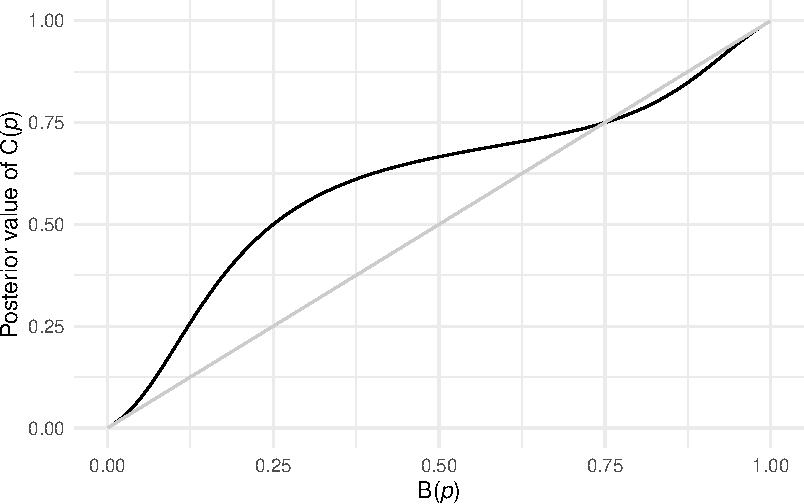
\includegraphics{defer-three_files/figure-pdf/fig-two-experts-1.pdf}

}

\caption{\label{fig-two-experts}The posterior probability of C(\emph{p})
given A(\emph{p})~=~0.75.}

\end{figure}%

The

\phantomsection\label{refs}
\begin{CSLReferences}{1}{0}
\bibitem[\citeproctext]{ref-Gallow2018}
Gallow, J. Dmitri. 2018. {``No One Can Serve Two Epistemic Masters.''}
\emph{Philosophical Studies} 175 (10): 2389--98. doi:
\href{https://doi.org/10.1007/s11098-017-0964-8}{10.1007/s11098-017-0964-8}.

\end{CSLReferences}



\noindent \vspace{1in} In progress

\end{document}
